\usetikzlibrary{decorations.pathreplacing, positioning}

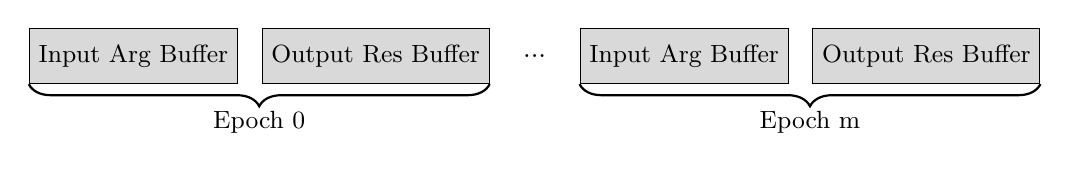
\begin{tikzpicture}[memoryblock/.style={draw, fill=gray!30, minimum width=3em, minimum height=2em, text centered, font=\small}, node distance=0.3cm]

	% Title

	% Epoch 0
	\node[memoryblock] (in0) at (0,1) {Input Arg Buffer};
	\node[memoryblock, right=0.3cm of in0] (out0) {Output Res Buffer};

	% Ellipsis for intermediate epochs
	\node[right=0.3cm of out0] (dots) {...};

	% Epoch m
	\node[memoryblock, right=0.3cm of dots] (inm) {Input Arg Buffer};
	\node[memoryblock, right=0.3cm of inm] (outm) {Output Res Buffer};

	% Braces for epochs
	\draw[decorate, decoration={brace,mirror,amplitude=8pt}, thick] (in0.south west) -- (out0.south east)
	node[midway,below=6pt, font=\small] {Epoch 0};

	\draw[decorate, decoration={brace,mirror,amplitude=8pt}, thick] (inm.south west) -- (outm.south east)
	node[midway,below=6pt, font=\small] {Epoch m};

\end{tikzpicture}

